\chapter{多态}

\section{多态}

\subsection{多态(Polymorphism)}

多态是同一个行为具有多个不同表现形式或形态的能力。

\begin{figure}[H]
	\centering
	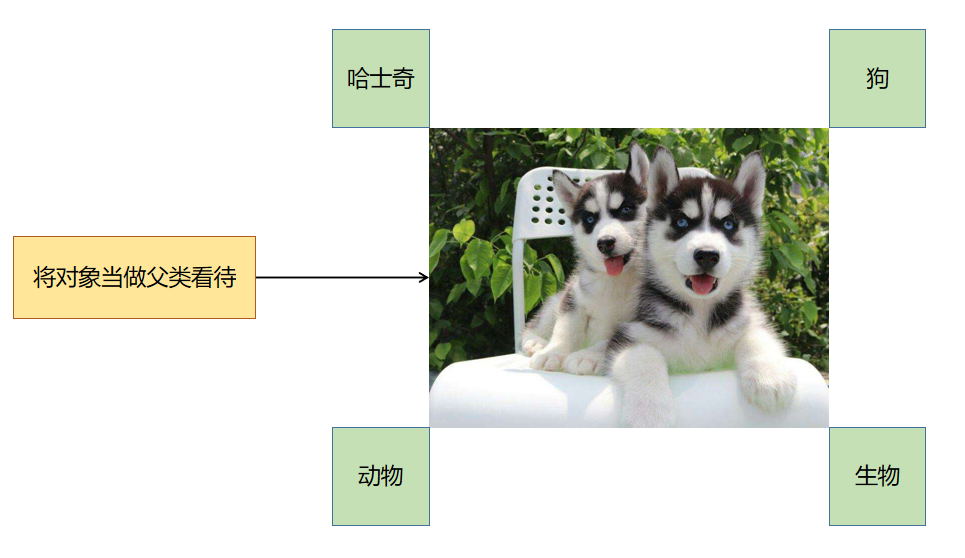
\includegraphics[scale=0.7]{img/C4/4-1/1.png}
	\caption{多态}
\end{figure}

\begin{figure}[H]
	\centering
	\begin{tikzpicture}[]
		\draw (0,0) node {Animal animal = new Dog();};

		\draw (-3,-2) rectangle (-1,-1);
		\draw (1,-2) rectangle (3,-1);
		\draw (-2,-1.5) node {父类引用};
		\draw (2,-1.5) node {子类对象};

		\draw[->] (-2,-1) -- (-1.5,-0.3);
		\draw[->] (2,-1) -- (1.5,-0.3);
	\end{tikzpicture}
	\caption{父类引用指向子类对象}
\end{figure}

通过父类引用指向子类对象,从而产生多种形态。父类引用仅能访问父类所声明的属性和方法,不能访问子类独有的属性和方法。\\

在一对有继承关系的类中都有一个方法,其方法名、参数列表、返回值均相同,通过调用方法实现不同类对象完成不同的事件。\\

构成多态需要满足三个条件:

\begin{enumerate}
	\item 必须存在继承关系。
	\item 继承关系中必须有同名的虚函数。
	\item 存在基类类型的指针或引用,通过该指针或引用调用虚函数。
\end{enumerate}

\newpage

\section{虚函数}

\subsection{虚函数}

虚函数是定义在基类中的函数,子类必须对其进行重写/覆盖(override),虚函数需要在类的成员函数前面加上virtual关键字。\\

重写/覆盖是指子类中存在重新定义的函数,其函数名、参数列表、返回值类型都与父类中被重写的函数一致。被重写的函数必须是虚函数。\\

子类若重写了父类的函数,那么子类将会隐藏其父类中被重写的函数。但是子类通过强制类型转换成父类后可以重新调用父类中被重写的函数。\\

\mybox{虚函数}

\begin{lstlisting}[language=C++, title=programmer.h]
#ifndef _PROGRAMMER_H_
#define _PROGRAMMER_H_

#include <string>

class Programmer {
public:
	Programmer(std::string title = "programmer");
	virtual void work();
	
private:
	std::string title;
};

#endif
\end{lstlisting}

\begin{lstlisting}[language=C++, title=programmer.cpp]
#include "programmer.h"
#include <iostream>

using namespace std;

Programmer::Programmer(string title) : title(title) {}

void Programmer::work() {
	cout << "programming" << endl;
}
\end{lstlisting}

\begin{lstlisting}[language=C++, title=java\_programmer.h]
#ifndef _JAVA_PROGRAMMER_H_
#define _JAVA_PROGRAMMER_H_

#include "programmer.h"
#include <string>

class JavaProgrammer : public Programmer {
public:
	JavaProgrammer(std::string title = "Java Programmer");
	virtual void work() override;
};

#endif
\end{lstlisting}

\begin{lstlisting}[language=C++, title=java\_programmer.cpp]
#include "java_programmer.h"
#include <iostream>

using namespace std;

JavaProgrammer::JavaProgrammer(string title) 
	: Programmer(title) {}

void JavaProgrammer::work() {
	cout << "Android Development" << endl;
}
\end{lstlisting}

\begin{lstlisting}[language=C++, title=test\_programmer.cpp]
#include <iostream>
#include "programmer.h"
#include "java_programmer.h"

using namespace std;

int main() {
	JavaProgrammer javaProgrammer;
	javaProgrammer.work();
	Programmer programmer = (Programmer)javaProgrammer;
	programmer.work();
	return 0;
}
\end{lstlisting}

\begin{tcolorbox}
	\mybox{运行结果}
	\begin{verbatim}
Android Development
programming
	\end{verbatim}
\end{tcolorbox}

\newpage

\section{纯虚函数}

\subsection{纯虚函数}

在虚函数后加上【= 0】后可以让这个函数变成纯虚函数,包含纯虚函数的类叫做抽象类(abstract class)或接口类(interface)。\\

抽象类不能被用于实例化对象,只是提供了所有的子类共有的部分。例如在动物园中,存在的都是动物具体的子类对象,并不存在动物对象,所以动物类不应该被独立创建成对象。\\

抽象类的作用是可以被子类继承,提供共性的属性和方法。父类提供的方法很难满足子类不同的需求,如果不定义该方法,则表示所有的子类都不具有该行为。如果定义该方法,所有的子类都在重写,那么这个方法在父类中是没有必要实现的,显得多余。\\

被virtual关键字修饰的方法称为纯虚函数。纯虚函数只有声明,没有实现。纯虚函数只能包含在抽象类中。产生继承关系后,子类必须重写父类中所有的纯虚函数,否则子类还是抽象类。\\

\mybox{纯虚函数}

\begin{lstlisting}[language=C++, title=shape.h]
#ifndef _SHAPE_H_
#define _SHAPE_H_

class Shape {
public:
	virtual double getArea() = 0;
};

#endif
\end{lstlisting}

\begin{lstlisting}[language=C++, title=rectangle.h]
#ifndef _RECTANGLE_H_
#define _RECTANGLE_H_

#include "shape.h"

class Rectangle : public Shape {
public:
	Rectangle(double length = 0, double width = 0);
	virtual double getArea() override;

private:
	double length;
	double width;
};

#endif
\end{lstlisting}

\begin{lstlisting}[language=C++, title=rectangle.cpp]
#include "rectangle.h"

Rectangle::Rectangle(double length, double width)
	: length(length), width(width) {}

double Rectangle::getArea() {
	return length * width;
}
\end{lstlisting}

\begin{lstlisting}[language=C++, title=circle.h]
#ifndef _CIRCLE_H_
#define _CIRCLE_H_

#include "shape.h"

class Circle : public Shape {
public:
	Circle(double raidus = 0);
	virtual double getArea() override;

private:
	double radius;
};

#endif
\end{lstlisting}

\begin{lstlisting}[language=C++, title=circle.cpp]
#include "circle.h"

Circle::Circle(double radius) : radius(radius) {}

double Circle::getArea() {
	return 3.14159 * radius * radius;
}
\end{lstlisting}

\begin{lstlisting}[language=C++, title=test\_shape.cpp]
#include <iostream>
#include "rectangle.h"
#include "circle.h"

using namespace std;

int main() {
	Rectangle rectangle(7, 5);
	Circle circle(6);
	cout << "rectangle: " << rectangle.getArea() << endl;
	cout << "circle: " << circle.getArea() << endl;
	return 0;
}
\end{lstlisting}

\begin{tcolorbox}
	\mybox{运行结果}
	\begin{verbatim}
rectangle: 35
circle: 113.097
	\end{verbatim}
\end{tcolorbox}

\vspace{0.5cm}

\subsection{接口(Interface)}

在面向对象中会使用抽象类为外部提供一个通用的、标准化的接口。\\

宏观上来讲,接口是一种标准。例如常见的USB接口,电脑通过USB接口连接各种外设设备,每一个接口不用关心连接的外设设备是什么,只要这个外设设备实现了USB的标准,就可以连接到电脑上。

\begin{figure}[H]
	\centering
	
\includegraphics[scale=0.4]{img/C4/4-3/1.png}
	\caption{USB接口}
\end{figure}

从程序上来讲,接口代表了某种能力和约定。当父类的方法无法满足子类需求时,可实现接口扩充子类的能力,接口中方法的定义代表能力的具体要求。\\

使用接口可以进行对行为的约束和规则的制定,接口表示一组能力,那么一个类可以接受多种能力的约束。因此一个类可以实现多个接口,实现多个接口的时候,必须要把每一个接口中的方法都实现。\\

\mybox{接口}

\begin{lstlisting}[language=C++, title=language.h]
#ifndef _LANGUAGE_H_
#define _LANGUAGE_H_

class Language {
public:
	virtual void translate() = 0;
};

#endif
\end{lstlisting}

\begin{lstlisting}[language=C++, title=english.h]
#ifndef _ENGLISH_H_
#define _ENGLISH_H_

#include "language.h"
#include <string>

class English : public Language {
public:
	English(std::string content = "");
	virtual void translate() override;

private:
	std::string content;
};

#endif
\end{lstlisting}

\begin{lstlisting}[language=C++, title=english.cpp]
#include "english.h"
#include <iostream>
#include <string>

using namespace std;

English::English(string content) : content(content) {}

void English::translate() {
	cout << content << endl;
}
\end{lstlisting}

\begin{lstlisting}[language=C++, title=chinese.h]
#ifndef _CHINESE_H_
#define _CHINESE_H_

#include "language.h"
#include <string>

class Chinese : public Language {
public:
	Chinese(std::string content = "");
	virtual void translate() override;

private:
	std::string content;
};

#endif
\end{lstlisting}

\begin{lstlisting}[language=C++, title=chinese.cpp]
#include "chinese.h"
#include <iostream>
#include <string>

using namespace std;

Chinese::Chinese(string content) : content(content) {}

void Chinese::translate() {
	cout << content << endl;
}
\end{lstlisting}

\begin{lstlisting}[language=C++, title=test\_language.cpp]
#include <iostream>
#include "language.h"
#include "english.h"
#include "chinese.h"

using namespace std;

void show(Language& language) {
	language.translate();
}

int main() {
	English english("Hello!");
	show(english);

	Chinese chinese("你好!");
	show(chinese);
	return 0;
}
\end{lstlisting}

\begin{tcolorbox}
	\mybox{运行结果}
	\begin{verbatim}
Hello!
你好
	\end{verbatim}
\end{tcolorbox}

\newpage